\chapter{Developer Documentation} % Developer guide
\label{ch:impl}

In this chapter, one might find relevant information and details regarding the architecture, implementations and testing of the tool. All of it helps to better understand how to change anything or what to do in order to apply it to your own application or a tool if one developer wants to borrow some use cases implementation in the visualizer. Main goal of the chapter is to clearly deliver the structure and preparation that has been made in the background of creation of a tool.

\section{Architecture}

One of the most crucial parts in the development is to have your architecture planned neatly and thoroughly in order to meet the resources one has in their hands. 

``At the heart of software architecture is the principle of abstraction: hiding some of the details of a system through encapsulation in order to better identify and sustain its properties.``~\cite{mshaw-data-knowledge}
	
By Shaw, software architecture is the abstraction for the end user, so that the certain details are hidden from them in order to keep everything clear and show the bigger picture of the things going under the hood of a software.

``The Unified Modeling Language (UML) is a graphical language for visualizing, specifying, constructing, and documenting the artifacts of a software-intensive system. The UML gives you a standard way to write a system's blueprints, covering conceptual things such as business processes and system functions, as well as concrete things such as classes written in a specific programming language, database schemas, and reusable software components.``~\cite{uml-user-guide} UML is used to better show the architectural decisions made as it is both popular and easy to read.

	
\subsection{Use cases}

On the figure 3.1 you might see the use case for the visualization tool. ``A use case is a prose description of a system's behavior when interacting with the outside world.``~\cite{alistair-human-and-technology} By following the definition of the Alistair, that he has introduced in his article, there are couple of moments on the such prose descriptions one might find there. 

So let's start with the so called "Actor", the entity which will represent the user of a tool and the set of actions that such user might use. In our case "Learner" is our "Actor" and the following actions are introduced: create graph, load prepared graph, control nodes, control edges, choose algorithm, control algorithm.

As one could deduce from the figure, there is a relation between the two actions - create graph and load prepared graph. Relation carries a name "Extend" as it represents the coupling of these actions. Create graph action logically contains the functionality which could be extended in order to implement load prepared graph action. 

\begin{figure}[H]
	\centering
	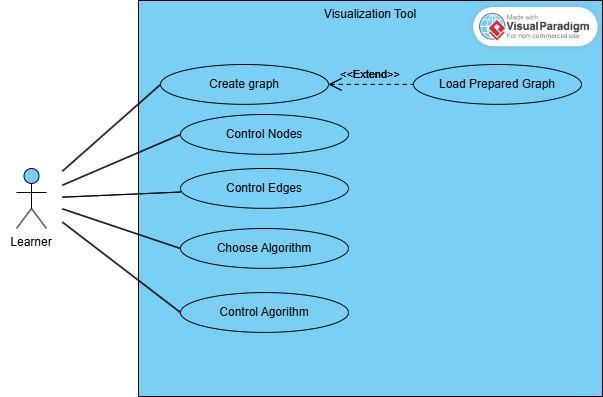
\includegraphics[width=\textwidth]{images/use_case_diagram.png}
	\caption{Use case diagram}
\end{figure}

\subsection{Component diagram}

Getting more concrete, developer might find a component diagram on figure 3.2. It explains the high-level design for the components of the tool that interacts with each other in order to achieve the desired result.

Components are the abstractions for the group of methods and classes working together to produce certain output. Though, they are related to each other not by their correspondence but by the end-goal they are created to achieve.

In case of the visualization tool, we have three main components, where one of them is coupled into the other. These are front end, back end and database. Due to the time limitations and initial decisions of the author of such tool, database is coupled into the back end and the mocked database basically inherits its interface. Meaning that the database is implemented in the same place as back end, with all of its methods. Though it may seem that it is a part of back end component, it is also true, that the database serves different purpose and applies different logic in itself. For this cause, there are not two, but three components which one could notice on the diagram.

Front end component serves as a "View" model and only accounts for the representation of data on the screen of the user. Main business logic behind all of data processing is made in the back end. Every time the client - front end - sends certain request to the back end, the latter processes it and send the ready response back to the client with all of the relevant data it may need. 

On this stage of the tool, it uses session-based storage. Session proceeds as long as the back end component is up, meaning that if the back end is down, all of the data is cleared up and it is not possible to restore the data. All due to the limitation of the mocked database, which simply stores the data inside of the data structure in the program such as maps, which causes it to store the data only during lifetime of the process.

\begin{figure}[H]
	\centering
	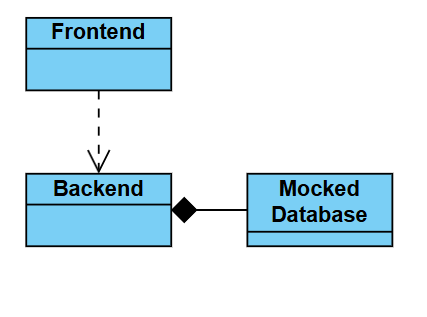
\includegraphics[width=\textwidth]{images/component_diagram.png}
	\caption{Component diagram}
\end{figure}

\subsection{Class diagram}

Figure 3.3 represents the class diagram of the application. It is not complete in a sense that it contains all of the classes that has been created during the development of the tool but it does contain the main classes that are worth mentioning so that the developer fully grasps the dependencies and coupling which occurs in the code.

View component abstracts all of the code in the front end as it does not contain any class hierarchy that would be necessary to show on the diagram due to its sole goal of representing data. Thus, the view components classes had been reduced to a single component element on the diagram.

``Web Server Gateway Interface, known as WSGI, is a specification that describes how a web server communicates with web applications, and how web applications can be chained together to process one request.``\cite{wsgi-def} In case of the visualization tool, it contains an implementation of WSGI which makes it possible for the client to access and influence the data through requests.

WSGI depends on "Response Handler" which does all of the work related to coupling all of the main logic of the application together. It aggregates the algorithm and graph classes, which it uses in order to patch responses. Though, it is important to say that it actually decouples the classes as it inverts the dependency to itself instead of having algorithm class anyhow coupled to the graph class. One of the main benefits of such decision is that the graph "component" now can be used freely and "shipped" with other components that might not need the algorithm "component" in them.

Graph and Algorithm interfaces help to abstract the types of theirs. There are six classes that implement them where undirected and directed graphs implement the graph interface whereas Bellman-Ford, Dijkstra, BFS, DFS classes implement the algorithm interface. By such decision, we introduce a new concept called inheritance. ``If an object is similar to another, (it has the same attributes and methods), then its class may be inherited from the classes of the similar objects: inherits their properties, and it might modify and augment them.``~\cite{oop-inheritance_def} The purpose of the inheritance is clarified now, as the classes have same properties.

\begin{figure}[H]
	\centering
	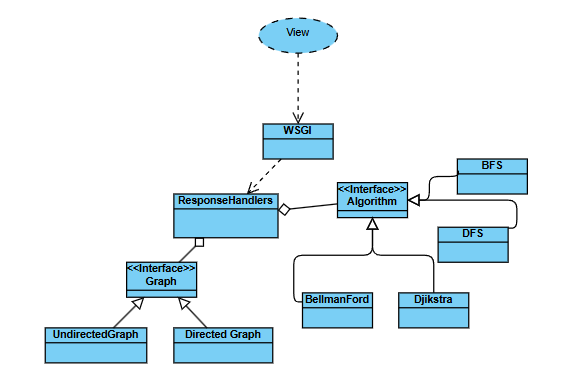
\includegraphics[width=\textwidth]{images/class_diagram.png}
	\caption{Class diagram}
\end{figure}

\subsection{Graph representation}

Graph representation is an important choice during the development of graphs. The decision on it may affect the future development of the algorithms, sometimes causing it to be less efficient. Two of the most popular choices are "Adjacency-list" and "Adjacency matrix". In case of the visualization tool, choice has been made in favor of an adjacency list representation.

Here are the definitions of these types by Cormen, ``The adjacency-list representation of a graph G=(V,E) consists of an array $Adj$ of $|V|$ lists, one for each vertex in $V$. For each $u \in V$, the adjacency list $Adj[u]$ contains all the vertices $v$ such that there is an edge $(u,v) \in E$. That is, $Adj[u]$ consists of all the vertices adjacent to $u$ in $G$. (Alternatively, it can contain pointers to these vertices.) The adjacency-matrix representation of a graph G=(V,E) assumes that the vertices are numbered $1,2,...,|V|$ in some arbitrary manner. Then the adjacency-matrix representation of a graph G consists of a $|V| \times |V|$ matrix $A = (a_{ij})$ such that``~\cite{cormen-introduction-to-algorithms}

\begin{math}
	a_{ij} = 
	\begin{cases}
		1		& \quad \text{if} (i,j) \in E\\
		0		& \quad \text{otherwise.}
	\end{cases}
\end{math}

\begin{figure}[H]
	\centering
	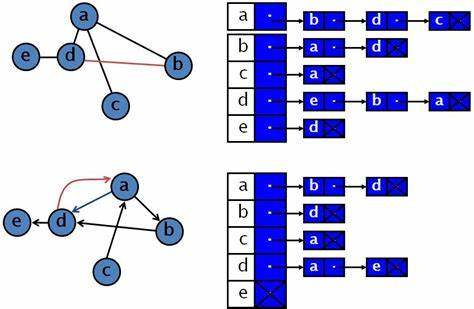
\includegraphics[width=120mm]{images/adjacency_list.jpg}
	\caption{Adjacency list representation}
\end{figure}

\begin{figure}[H]
	\centering
	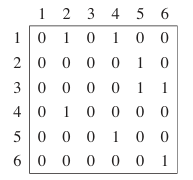
\includegraphics[width=80mm]{images/matrix_representation.png}
	\caption{Adjacency matrix representation}
\end{figure}

\section{Technical details}

So that one could clearly comprehend what is happening in the code and why such decisions had been made, they must know the technical details behind the code.

\subsection{Libraries}

Decision on the libraries made a big role in the complexity of developing the tool. Some of them made things harder to implement, some of them reduced a lot of work that could have been done if they were not used. Though it is fair to mention that nothing is perfect and when it comes to the choice of libraries used in development, it is no different. You have to deal with the limitations of certain libraries and at times go through the places you have never expected yourself to be in. 

Here are the main libraries that have been used in development of the tool, both in front and back ends.

\subsubsection{React JS}

As one of the main library for the development of the user end, the React has been chosen. Some definitions from its github page:

``React is a JavaScript library for building user interfaces.``~\cite{react-github}

``Declarative: React makes it painless to create interactive UIs. Design simple views for each state in your application, and React will efficiently update and render just the right components when your data changes. Declarative views make your code more predictable, simpler to understand, and easier to debug.``~\cite{react-github}

``Component-Based: Build encapsulated components that manage their own state, then compose them to make complex UIs. Since component logic is written in JavaScript instead of templates, you can easily pass rich data through your app and keep the state out of the DOM.``~\cite{react-github}

The library is popular among the developers, especially the ones, who specifically create client-side applications. Choice came to it, as there were loads of tutorials and templates to learn from, though it did not make it easy to learn. It was one of the choices, which consumed a lot of time just on the phase of learning it. Are there any regrets? No, there was a lot to learn and grasp, one could only be glad to know so much things, and certainly, after learning it, you most probably will know it.

\subsubsection{React-bootstrap}

Though React is a good choice for the front, one could not achieve an easy UI development without such library as react-bootstrap.

``React-Bootstrap is a complete re-implementation of the Bootstrap components using React. It has no dependency on either bootstrap.js or jQuery.``~\cite{react-bootstrap}

It helped a lot during the development of the tool, as it self-contains a great amount of ready templates and it significantly decreases the time one needs to spend on developing the UI.

\subsubsection{React-d3-graph}

React-d3-graph is the library used for drawing a graph on ones page. It is build on top of another JavaScript library, which is d3.js. ``D3 (or D3.js) is a free, open-source JavaScript library for visualizing data. Its low-level approach built on web standards offers unparalleled flexibility in authoring dynamic, data-driven graphics. For more than a decade D3 has powered groundbreaking and award-winning visualizations, become a foundational building block of higher-level chart libraries, and fostered a vibrant community of data practitioners around the world.``~\cite{d3-js} 

D3 solves wide range of problems, while react-d3-graph gathers everything you need to deal with graphs. For this very reason, it is decided to be an optimal choice as there would be no need in having access to all of the features of D3 library, as it would bring nothing but increased complexity. 

It is trivial to choose abstractions when you have a choice.

\subsubsection{React-query}

One last library that has been used alongside react is react-query. It helped in reducing the number of hook usage such as useEffect and useState, making it more maintainable and bugs resistant.

``TanStack Query (FKA React Query) is often described as the missing data-fetching library for web applications, but in more technical terms, it makes fetching, caching, synchronizing and updating server state in your web applications a breeze.``~\cite{react-query-web}

Basically, in the application, only two hooks from the library have been used which are useMutation and useQuery. However, these two hooks has replaced with itself huge amount of repetitive code that resided in the application with just the usage of useEffect hook. The impact of this library on the development process has been crucial.

\subsubsection{HTML}

``HTML (HyperText Markup Language) is the most basic building block of the Web. It defines the meaning and structure of web content. "Hypertext" refers to links that connect web pages to one another, either within a single website or between websites. Links are a fundamental aspect of the Web. By uploading content to the Internet and linking it to pages created by other people, you become an active participant in the World Wide Web.``~\cite{html-def}

Static HTML has not been used widely, rather a single instance is used to run the whole web page on. It is all possible due to the way react renders the application.

\subsubsection{Python Flask}

``Flask is a web framework that allows developers to build lightweight web applications quickly and easily with Flask Libraries. It was developed by Armin Ronacher, leader of the International Group of Python Enthusiasts(POCCO). It is basically based on the WSGI toolkit and Jinja2 templating engine.``~\cite{flask-def}

Whole back end site of the application is built using python. Logic of the graphs and algorithms, response handlers and database, though all of it would not make sense without a proper way of establishing a communication between two ends. Flask is making it possible by giving the developer a WSGI where one could list his endpoints.

\section{Implementations}

By this part of the documentation, one has to gain enough of information in order to understand the implementation of  code. Indeed, a reasonable background is needed as well. 

Front end related code is not going to be covered as it is simply of no need, to show how the application "shows" itself, rather the business logic code and endpoints are going to be exposed to the developer for the sake of clarification. 

\subsection{API endpoints}

Server envelops the following api endpoints in itself.

\begin{itemize}
	\item GET - get graph, get database
	\item POST - import graph from file, add node, add edge, add edge with weight, run algorithm
	\item DELETE - clear graph, remove node, clear algorithm, remove edge
	\item PUT - set graph type, set weight, change algorithm, do step
\end{itemize}

By calling these endpoints, the developer might change the data and get the changed data as a response, in order to use it. This is how the client side of the application works, calling the data, receiving, "showing".

\subsection{Graph management}

Let's see how some of the main endpoints actually get the graph data or manage it in case of a modification request.

\subsubsection{Getting graph}

First of all, the endpoint method declared in the WSGI calls for a graph response handler's method get graph, which will return the parsed response, it also appends the data of the current algorithm if there is such and sends back the prepared response.

\lstset{caption={Get graph endpoint}, label=fig:get-graph-endpoint}
\begin{lstlisting}[language={python}]
	@app.route("/graph", methods=["GET"])
	def get_graph():
		response = GraphResponseHandler.get_graph()
		response.update(AlgorithmResponseHandler.get_algorithm())
		return jsonify(response)
\end{lstlisting}

Going deeper, get graph method of the graph response handler will call the database through, so-called, session storage that stores current graph, algorithm and database, and get the graph table in it. After that, it just sends back the ready graph data.

\lstset{caption={Get graph method in response handler}, label=fig:get-graph-method-in-response-handler}
\begin{lstlisting}[language={python}]
 	@staticmethod
	def get_graph():
		graph_data = {'graph': Storage.database.get_table('graph')}
		if graph_data['graph'] == {}:
			graph_data.update({'nodes': [], 'edges': {}})
		return graph_data
\end{lstlisting}

\subsubsection{Changing graph}

As we have two main types of graph, we have an endpoint for this use case as well. All it takes is a name of the graph and passes down the responsibility to the response handler. 

The method of the response handler on code field 3.3, checks whether the provided type name is not the same as the one that is already in use. After the check, it calls session storage's method change graph.

\lstset{caption={Change graph type}, label=fig:graph-type-change}
\begin{lstlisting}[language={python}]
    @staticmethod
	def set_graph_type(graph_type_name):
		if isinstance(Storage.graph, graph_types.get(graph_type_name)().__class__):
			return {'msg': f'Graph is already of type - {graph_type_name}'}
		Storage.change_graph(graph_types.get(graph_type_name)())
		return GraphResponseHandler._update_database_data()
\end{lstlisting}

In the session storage, one might see that it does nothing other than initializing graph in use to the new graph instance. Which means, that the previous graph will be garbage collected with its fields.

One way to get the instance of certain class by its name is application of the factory-like design pattern. Graph factory class employs this design pattern yet, with some modifications included in it. Graph type dictionary actually makes it possible to create certain instances by their names.

\lstset{caption={Change graph in storage}, label=fig:graph-type-storage}
\begin{lstlisting}[language={python}]
 	@staticmethod
	def change_graph(new_graph):
		Storage.graph = new_graph
\end{lstlisting}

\lstset{caption={Graph Factory}, label=fig:graph-factory}
\begin{lstlisting}[language={python}]
	class GraphFactory:
		@staticmethod
		def create_UndirectedGraph():
			return UndirectedGraph()
		
		@staticmethod
		def create_DirectedGraph():
			return DirectedGraph()
	
	
	graph_types = {
		'undirected': GraphFactory.create_UndirectedGraph,
		'directed': GraphFactory.create_DirectedGraph,
	}
\end{lstlisting}

\subsubsection{Importing graph from file}

Rest of the endpoints do pretty much the same thing as the previous endpoint does. Import graph from file endpoint takes graph file index and calls the response handler to handle it.

As shown on the figure 3.6 under the persistence folder in the src, we have the graph templates. There the numbers appended at the end of each one corresponding to their index.

\begin{figure}[H]
	\centering
	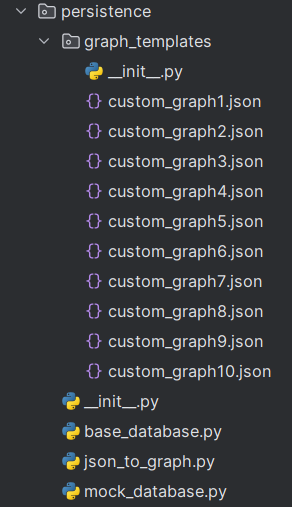
\includegraphics[width=80mm]{images/custom_graphs.png}
	\caption{Custom graphs}
\end{figure}

\lstset{caption={Custom graph template}, label=fig:custom-graph-template}
\begin{lstlisting}[language={Xml}]
	{
		"graph": {
			"nodes" : [0, 1, 2, 3, 4],
			"edges" : [
			[[1, 1]],
			[[2, -10], [3, 1]],
			[[4, 1]],
			[],
			[[3, 9]]
			]
		}
	}
\end{lstlisting}

Response handler, in its method, looks for the file with the corresponding index, after which it sends the file it found down to the JsonToGraph class and its method json to graph. At the end, after initializing parsed graph to the one in the storage, method sends the updated data back.

\lstset{caption={Import ready graph response handler}, label=fig:import-ready-graph-response-handler}
\begin{lstlisting}[language={python}]
 	@staticmethod
	def import_ready_graph(index_of_graph):
		dirs_to_find = ['app', 'src', 'persistence', 'graph_templates']
		path = os.getcwd()
		graph_file_name = 'custom_graph' + str(index_of_graph) + '.json'
		while len(directory := os.listdir(path)) > 0:
			if graph_file_name in directory:
				path += os.sep + graph_file_name
				break
		
			any_path_found = False
			for _dir in directory:
				if _dir in dirs_to_find:
					path += os.sep + _dir
					any_path_found = True
					break
		
			if not any_path_found:
				break
		
		path_to_graph_file = path
		Storage.graph = JsonToGraph.json_to_graph(path_to_graph_file, Storage.graph.__class__)
		return GraphResponseHandler._update_database_data()
\end{lstlisting}

Json to graph method in its turn, read the data from a file and creates a new graph of the type that the previous graph had. 

Here one could see the beneficial parts of the interfaces, where the code uses the graphs methods add edge and add node without caring whether it will work the way the method needs it to work. Graph interface brings with itself the simplification to the code.

\lstset{caption={Json to graph method}, label=fig:json-to-graph-method}
\begin{lstlisting}[language={python}]
	@staticmethod
	def json_to_graph(json_path, class_of_graph):
		with open(json_path, 'r') as json_file:
			json_dict = json.load(json_file)
		if class_of_graph is UndirectedGraph:
			new_graph = UndirectedGraph()
		else:
			new_graph = DirectedGraph()
		
		json_dict = json_dict['graph']
		for _ in json_dict['nodes']:
			new_graph.add_node()
		
		index = 0
		for edges_of_node in json_dict['edges']:
			for edge in edges_of_node:
				new_graph.add_edge(new_graph.nodes[index], new_graph.nodes[edge[0]], edge[1])
			index += 1
		
		return new_graph
\end{lstlisting}

\subsubsection{Addition of node}

The method of adding a node is the same for both undirected and directed graphs. Also, there is nothing complicated going on, just the creation of a node and appending of it to the list of nodes and edges, after all of which, we return the node.

\lstset{caption={Adding node}, label=fig:adding-node}
\begin{lstlisting}[language={python}]
 	def add_node(self) -> Node:
		new_node = Node()
		self.nodes.append(new_node)
		self.edges.append([])
		return new_node
\end{lstlisting}

Node class is more interesting as it consists of two useful features, that one could call a "constructor" and a "deconstructor". Each node has a unique id that identifies it on the graph, as you could see already in the user documentation. All of it comes from here, where during the initialization of the node, it calls the node id generators method, which generates the id for the node, and safes it in itself. 

On code 3.10, the developer might see that it calls for its method of id generation, and saves the hash of the node object, lastly, increasing the count of nodes. It is saving the hash of the object due to the requirements of the garbage collector which checks whether the object is being referenced anywhere in the code and calls for its deconstructor only when it does not.

\lstset{caption={Node class}, label=fig:node-class}
\begin{lstlisting}[language={python}]
	class Node:
		def __init__(self):
			NodeIDGenerator.generate_id_node_pair(self)
		
		def __del__(self):
			NodeIDGenerator.remove_id_of_node(self)
\end{lstlisting}

\lstset{caption={Generating ids for nodes}, label=fig:node-id-generation}
\begin{lstlisting}[language={python}]
    @staticmethod
	def generate_id_node_pair(node):
		new_id = NodeIDGenerator.generate_id()
		NodeIDGenerator.ids_and_nodes[new_id] = node.__hash__()
		NodeIDGenerator.node_count += 1
\end{lstlisting}


\subsubsection{Removal of node}

Removal of node is more complicated compared to the addition, due to its need to check the edges outgoing from it and incoming into it. Developer can see it on code 3.12 where it does the exact thing mentioned in the previous sentence, though it is not all of the work that is done, as we will have the garbage collector call the deconstructor on the node as it is no longer in use.

\lstset{caption={Remove node in graph}, label=fig:remove-node}
\begin{lstlisting}[language={python}]
 	def remove_node(self, index):
		self.nodes.pop(index)
		self.edges.pop(index)
		
		for edge in self.edges:
			index_to_pop = -1
			for i in range(len(edge)):
				if edge[i][0] == index:
					index_to_pop = i
			if index_to_pop != -1:
				edge.pop(index_to_pop)
			for i in range(len(edge)):
				if edge[i][0] > index:
					edge[i][0] -= 1
\end{lstlisting}

When it comes to the deconstructor, it calls the id generators method - remove id of node. Getting the node instance, it finds its id and deletes its instance, then shifting all of the hashes one to the left, it deletes its hash from the id generator as well.

\lstset{caption={Id removal of node}, label=fig:remove-node-id}
\begin{lstlisting}[language={python}]
 	@staticmethod
	def remove_id_of_node(node):
		id = NodeIDGenerator.get_id_of_node(node)
		NodeIDGenerator.remove_id(id)
		for key in range(id, NodeIDGenerator.node_count-1):
			NodeIDGenerator.ids_and_nodes[key] = NodeIDGenerator.ids_and_nodes[key+1]
		NodeIDGenerator.ids_and_nodes.pop(NodeIDGenerator.node_count - 1)
		NodeIDGenerator.node_count -= 1
\end{lstlisting}

\subsubsection{Addition of edge}

Addition of edge is implemented in the simplest way possible. Method checks whether there is an edge between nodes, finding these nodes' indexes and adding them to each others' adjacency list.

\lstset{caption={Adding edge}, label=fig:add-edge}
\begin{lstlisting}[language={python}]
 	def add_edge(self, first_node, second_node, weight=0):
		if not (first_node in self.nodes or second_node in self.nodes):
			raise InvalidNodeException("One of the nodes in the edge is not in the nodes set.")
		first_node_index = self.nodes.index(first_node)
		second_node_index = self.nodes.index(second_node)
		self.edges[first_node_index].append([second_node_index, weight])
		self.edges[second_node_index].append([first_node_index, weight])
\end{lstlisting}

\subsubsection{Removal of edge}

To remove the edge, first we check for the edge cases, when one of the nodes does not exist, then we check whether there is an edge between the nodes. After couple of checks, we find the nodes in the list and each others adjacency list, then we remove them from both.

\lstset{caption={Removing edge, undirected}, label=fig:remove-edge-un}
\begin{lstlisting}[language={python}]
	def remove_edge(self, first_node, second_node):
		if not (first_node in self.nodes or second_node in self.nodes):
			raise InvalidNodeException("One of the nodes in the edge is not in the nodes set.")
		first_node_index = self.nodes.index(first_node)
		second_node_index = self.nodes.index(second_node)
		if not (second_node_index in [node[0] for node in self.edges[first_node_index]] or
		first_node_index in [node[0] for node in self.edges[second_node_index]]):
			raise InvalidNodeException("There is no edge between the nodes")
		first_to_second_edge_index = [node[0] for node in self.edges[first_node_index]].index(second_node_index)
		second_to_first_edge_index = [node[0] for node in self.edges[second_node_index]].index(first_node_index)
		self.edges[first_node_index].pop(first_to_second_edge_index)
		self.edges[second_node_index].pop(second_to_first_edge_index)
\end{lstlisting}

In case of a directed graph, we remove only one edge. The one outgoing from the first node to the second one. Indeed, some checks are required to be done beforehand.

\lstset{caption={Removing edge, directed}, label=fig:remove-edge}
\begin{lstlisting}[language={python}]
    def remove_edge(self, first_node, second_node):
	if not (first_node in self.nodes or second_node in self.nodes):
		raise InvalidNodeException("One of the nodes in the edge is not in the nodes set.")
	first_node_index = self.nodes.index(first_node)
	second_node_index = self.nodes.index(second_node)
	if not (second_node_index in [node[0] for node in self.edges[first_node_index]]):
		raise InvalidNodeException("There is no edge between the edges")
	first_to_second_edge_index = [node[0] for node in self.edges[first_node_index]].index(second_node_index)
	self.edges[first_node_index].pop(first_to_second_edge_index)
\end{lstlisting}

\subsubsection{Setting weight}

Each edge represents carries certain weight, by default it is 0. In case one want to make the graph truly "weighted", there is a need in setting the weight for edges.

Such an option is available in the tool and the endpoint resembles edge managing endpoints. It gets three inputs: edge incoming node, edge outgoing node and weight, so that it can find the corresponding edge and set the weight of it.

As one might see on figure 3.14, initially it checks whether there is such edge incoming node and edge outgoing node in the graph, then it finds those nodes indexes in the graph and each others adjacency list, in case of undirected graph, as the next step it sets the weight of edges to the one that has been passed as a parameter. If one would have to deal with directed graph, the method would be similar to the one on figure 3.14, the only difference is that we set the weight only for the edge from the edge outgoing node to edge incoming node.

\lstset{caption={Setting weight for the edge}, label=fig:setting-weight}
\begin{lstlisting}[language={python}]
 	def set_weight(self, first_node, second_node, weight):
		if not (first_node in self.nodes or second_node in self.nodes):
			raise InvalidNodeException("One of the nodes in the edge is not in the nodes set.")
		first_node_index = self.nodes.index(first_node)
		second_node_index = self.nodes.index(second_node)
		second_node_in_first_nodes_index = [node[0] for node in self.edges[first_node_index]].index(second_node_index)
		first_node_in_second_nodes_index = [node[0] for node in self.edges[second_node_index]].index(first_node_index)
		
		self.edges[first_node_index][second_node_in_first_nodes_index][1] = weight
		self.edges[second_node_index][first_node_in_second_nodes_index][1] = weight
\end{lstlisting}

\subsection{Algorithm management}

As one could have noticed already, the get graph method appends the algorithm data to the response as well. So in this section, all of the main information regarding the algorithms are going to be covered. 

\subsubsection{Changing algorithm}

There are four types of algorithm which you can change calling the relevant endpoint. It works pretty much the same way as change graph endpoint. Method initializes new algorithm instance which it creates using the algorithm factory. After that, it get the description of such algorithm and sends back the updated data as a response. 

The developer can find the algorithm factory on code 3.19 and the corresponding response handler on code 3.18.

\lstset{caption={Choose algorithm handler}, label=fig:choose-algo-handler}
\begin{lstlisting}[language={python}]
    @staticmethod
	def choose_algorithm(algorithm_name):
		Storage.change_algorithm(algorithm_names.get(algorithm_name))
		updated_table = Storage.database.get_tables().get('algorithm', {})
		updated_table.update({'description': Storage.algorithm.description()})
		return AlgorithmResponseHandler._update_database_data(updated_table)
\end{lstlisting}

\lstset{caption={Algorithm factory}, label=fig:algo-factory}
\begin{lstlisting}[language={python}]
	algorithm_names = {
		'dfs': AlgorithmFactory.create_DFS(),
		'bfs': AlgorithmFactory.create_BFS(),
		'dijkstra': AlgorithmFactory.create_Dijkstra(),
		'bellmanford': AlgorithmFactory.create_BellmanFord()
	}
\end{lstlisting}

\subsubsection{Starting algorithm}

One can start the algorithm by querying run algorithm endpoint of the tool. Then the endpoint call for the handler, which in its turn, runs it on the algorithm which it keeps in the session storage. 
As we have all of the algorithms classes derive a single algorithm abstract base class, we don't need to deal with handling of the specific algorithms methods being run. After that, we check whether the path has been found, and if not, we update the results dictionary object correspondingly. At the end, we send the final results as we append the description of the algorithm to the results.

\lstset{caption={Running algorithm method}, label=fig:run-algo}
\begin{lstlisting}[language={python}]
 	@staticmethod
	def run_algorithm(source, target):
		algorithm_data = Storage.algorithm.run(Storage.graph.edges, source, target)
		if algorithm_data['path'] == Storage.algorithm.PATH_NOT_FOUND:
			algorithm_data.update({'currentStep': -1, 'currentState': FINISHED_STATE})
		else:
			algorithm_data.update({'currentStep': 0, 'currentState': RUNNING_STATE})
		algorithm_data.update({'description': Storage.algorithm.description()})
		
		return AlgorithmResponseHandler._update_database_data(algorithm_data)
\end{lstlisting}

For the sake of clarification, one might want to look into code 3.21. It is a run method of a BFS algorithm, which actually traverses the graph and gives back the result. The algorithm itself is not in its original form. Usually, BFS just traverses the whole graph, but in this implementation it stops, when it finds the first path to the target node. Yet it is not wrong, it is still important to highlight. BFS algorithm in the tool is implemented with the usage of queue abstract data structure, which is also has been implemented by the author. 

All of the algorithms implement well-known patterns and there is no difference between them, with the exception of The Bellman-Ford, where it appends the isBellmanFord boolean value to the result, identifying that it needs to be handled in a different manner.

\lstset{caption={Algorithm's run method}, label=fig:run-algo-method}
\begin{lstlisting}[language={python}]
    def run(self, graph, source, target):
		if source is None or target is None:
			return {'path': Algorithm.PATH_NOT_FOUND, 'steps': []}
		path = []
		queue = Queue()
		queue.push((source, [source]))
		visited = [False] * (len(graph) + 1)
		
		while not queue.empty():
			(current_node, current_path) = queue.pop()
			if visited[current_node]:
				continue
			path.append(current_node)
			visited[current_node] = True
			if current_node == target:
				return {'path': current_path, 'steps': path}
			
			for node in sorted(graph[current_node]):
				if not visited[node[0]]:
					queue.push((node[0], current_path + [node[0]]))
		
		return {'path': Algorithm.PATH_NOT_FOUND, 'steps': path}
\end{lstlisting}

\subsubsection{Going through steps of algorithm}

Moving on through the methods of algorithm, developer might see the do step method on code 3.22, where the aforementioned isBellmanFord value could be noticed.

The method, as a first step, checks whether the algorithm it is running is the Bellman-Ford or not.

When it is not, it checks whether it is a last step or not, if it is, then we finish the algorithm, if not, in this case we increase the step index.

Though, in case it is actually the Bellman-Ford algorithm, we look whether it is a last edge, in other words link, to be checked and apply according changes to the result.

In the end, it sends the updated data back.

\lstset{caption={Algorithm step method}, label=fig:do-step}
\begin{lstlisting}[language={python}]
    @staticmethod
	def do_step():
		updated_table = Storage.database.get_tables().get('algorithm', {})
		if updated_table.get('isBellmanFord', '') == 'True':
			if updated_table['currentLink'] >= len(updated_table['links']) - 1 or updated_table['currentLink'] == -1:
				updated_table.update({'currentLink': -1, 'currentState': FINISHED_STATE})
			else:
				updated_table.update({'currentLink': (updated_table['currentLink'] + 1)})
		else:
			if updated_table['currentStep'] >= len(updated_table['steps']) - 1:
				updated_table.update({'currentStep': -1, 'currentState': FINISHED_STATE})
			else:
				updated_table.update({'currentStep': (updated_table['currentStep'] + 1)})
		return AlgorithmResponseHandler._update_database_data(updated_table)
\end{lstlisting}

\section{Testing}

Testing is and has played a crucial role in the development. The Test-Driven Development has been used throughout the process and for this cause, there are over a hundred of tests written.

``Test-driven development (TDD) is a method of coding in which you first write a test and it fails, then write the code to pass the test of development, and clean up the code. This process recycled for one new feature or change. In other methods in which you write either all the code or all the tests first, TDD will combine and write tests and code together into one.``~\cite{geeksforgeeks-tdd-def} Though it might seem that it slows the developing process, it actually prevents from making mistakes in the future. Also, with the CI written for the repository, it helped to avoid further problems a lot of times in the process.

\lstset{caption={CI yaml file}, label=fig:ci-yaml}
\begin{lstlisting}[language=yaml]
	---
	name: CI
	
			push:
				branches: [ "master" ]
		
			workflow_dispatch:
		
		jobs:
			test:
				runs-on: ubuntu-latest
		
				steps:
					- uses: actions/checkout@v4
					- uses: actions/setup-python@v5
					with:
						python-version: '3.12' 
		
					- name: install dependencies
					run: pip install -r app/requirements.txt
					- name: Create env file
					run: |
					pwd
					echo "PYTHONPATH=/home/runner/work/PathFinding/PathFinding" >> $GITHUB_ENV
					cat $GITHUB_ENV
					- name: set up environment and run tests
					run: python3 -v app/main.py &
					- name: Run the tests
					run: python3 -m unittest discover -v app/src/tests
		

			build:
				runs-on: ubuntu-latest
		
				steps:
					- uses: actions/checkout@v4
		
					- name: Run a one-line script
					run: echo Hello, world!
		
					- name: Run a multi-line script
					run: |
					echo Add other actions to build,
					echo test, and deploy your project.
	---
\end{lstlisting}

\subsection{Tests structure}

On figure 3.7, a folder is shown, which contains all of the test suites. They are separated into two main groups - unit tests and E2E tests. 

``Unit testing is a type of software testing that focuses on individual units or components of a software system. The purpose of unit testing is to validate that each unit of the software works as intended and meets the requirements.``~\cite{gfg-unit-test-def} 

On the other hand, E2E does pretty much the same, except for some detail. E2E tests send requests to the server-side and validates the responses. For this reason, E2Es are mostly slower and take more effort in debugging, as you would need an environment for that. Though, the E2E tests are inevitable when one deals with the endpoints in the system.

\begin{figure}[H]
	\centering
	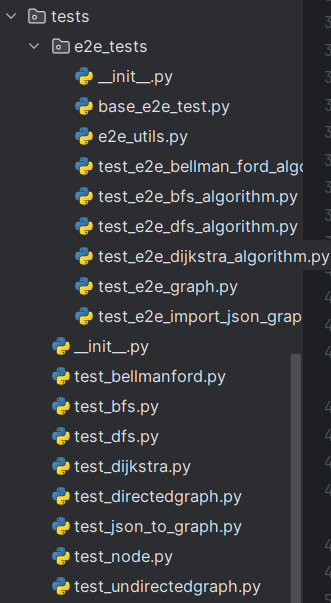
\includegraphics[width=80mm]{images/tests_folder.png}
	\caption{Tests folder}
\end{figure}

\subsection{Tests implementation}

As reviewing hundred tests would probably take around fifty pages to describe, here are some of the crucial and complex test cases. Starting with the unit tests, then E2E tests will help one see the correlation and differences between two ways of testing.

As can be seen on code 3.24, there are three parts of the test: given, when and then. This structure helps us to maintain clear and readable test methods and it also makes it easier to refactor.

In the node test, we see that some nodes are being created and removed after. This test makes sure that after the deconstructor is called on the node instance, it actually removes the necessary data.

\lstset{caption={Node test}, label=fig:node-test}
\begin{lstlisting}[language={python}]
	def test_create_and_delete_multiple_times(self):
		# given-when
		for i in range(10):
			self.nodes.append(Node())
			self.nodes.pop(i)
			self.nodes.append(Node())
		
		# then
		self.assertEqual(len(self.nodes), 10)
		for i in range(0, len(self.nodes)):
			self.assertEqual(NodeIDGenerator.ids[i], i)
			self.assertIn(i, NodeIDGenerator.ids_and_nodes.keys())
			self.assertEqual(NodeIDGenerator.ids_and_nodes[i], self.nodes[i].__hash__())
\end{lstlisting}
    
The graph test on code 3.25 is pretty long, yet it is purpose is straight. It tries to remove the nodes with the edges between each other, starting from the node, that is in the middle of the other two. 
Initially, the test creates the nodes and connects them in the given part. As one can see, the middle node is the second node in the test. After that, we can see multiple whens and thens going after each other, where we remove the middle node first, then the first one and at the end, we delete the remaining node, all of that while testing that the behavior of deleting a node is not deviating and not causing an undefined behavior.
    
\lstset{caption={Undirected graph test}, label=fig:graph-test}
\begin{lstlisting}[language={python}]
	def test_remove_three_nodes_with_edges_between_starting_from_middle(self):
	# given
	node1 = self.graph.add_node()
	node2 = self.graph.add_node()
	node3 = self.graph.add_node()
	
	self.graph.add_edge(node1, node2)
	self.graph.add_edge(node2, node3)
	
	# when
	self.graph.remove_node(NodeIDGenerator.get_id_of_node(node2))
	del node2
	
	# then
	self.assertEqual([NodeIDGenerator.get_id_of_node(node) for node in self.graph.nodes], [0, 1])
	self.assertEqual(len(self.graph.nodes), 2)
	self.assertEqual(len(self.graph.edges), 2)
	for edge in self.graph.edges:
	self.assertEqual(len(edge), 0)
	
	# when
	self.graph.remove_node(NodeIDGenerator.get_id_of_node(node1))
	del node1
	
	# then
	self.assertEqual([NodeIDGenerator.get_id_of_node(node) for node in self.graph.nodes], [0])
	self.assertEqual(len(self.graph.nodes), 1)
	self.assertEqual(len(self.graph.edges), 1)
	
	# when
	self.graph.remove_node(NodeIDGenerator.get_id_of_node(node3))
	del node3
	
	# then
	self.assertEqual(len(self.graph.nodes), 0)
	self.assertEqual(len(self.graph.edges), 0)
\end{lstlisting}

Compared to its E2E alternative, its quite huge. Yet it is obvious, that if we have the correct behavior in the unit tests, it must not be different for the E2E tests. Rather it tests the endpoint itself. The purpose of this E2E test is to make sure, that the endpoints trigger necessary places in the code.

\lstset{caption={Undirected graph E2E test}, label=fig:graph-e2e-test}
\begin{lstlisting}[language={python}]
 	def test_remove_node(self):
		# given
		UndirectedGraphE2ETest._request_add_node()
		node_id = 0
		
		# when
		requests.delete(f'http://127.0.0.1:5000/node/{node_id}').json()
		graph = self._get_graph()
		
		# then
		self.assertEqual(graph.get('graph'), EXPECTED_GRAPHS[0].get('graph'))
\end{lstlisting}
    
At last, the algorithm tests are taking an important part in the application, as they make sure that they are correct. Though, they would not perfectly identify whether the algorithm is valid or not, it would greatly reduce the chances of getting it wrong.

As an example, in the BFS test on code 3.27, it creates a graph and then runs an algorithm on it. In the end, checking its correctness, the test makes sure that it works for such sparse graphs.

\lstset{caption={BFS algorithm test}, label=fig:algo-test}
\begin{lstlisting}[language={python}]
    def test_multiple_node_sparse_connected_graph(self):
		# given
		for i in range(10):
			new_node = self.graph.add_node()
			if i > 0:
				self.graph.add_edge(new_node, self.graph.nodes[i-1])
		
		node_id1 = self._get_node_id(0)
		node_id2 = self._get_node_id(9)
		
		# when
		path = self.bfs.run(self.graph.edges, node_id1, node_id2).get('path')
		
		# then
		self.assertEqual(path, [self._get_node_id(i) for i in range(len(self.graph.nodes))])
\end{lstlisting}

In case of an E2E alternative of the test, it checks whether the next step endpoint is working properly and it returns the values that are expected from it. Significant part of such tests is having an expected output which one could actually deduct as correct solely by looking into it, without usage of external help. It helps to build tests based on those expectations and debug them later, if there is anything going not the way it is supposed to.

\lstset{caption={BFS algorithm E2E test}, label=fig:algo-e2e-test}
\begin{lstlisting}[language={python}]
    def test_multiple_node_connected_graph(self):
		# given
		for i in range(10):
			TestE2EBFSAlgorithm._request_add_node()
			if i > 0:
				requests.post(f'http://127.0.0.1:5000/edges/{i}/{i-1}')
		
		# when
		response = requests.post('http://127.0.0.1:5000/algorithm/0/9').json()
		gathered_steps = [response['algorithm']['currentStep']]
		while ((response := requests.put('http://127.0.0.1:5000/algorithm/next_step').json())
		.get('algorithm').get('currentState') == RUNNING_STATE):
			gathered_steps.append(response['algorithm']['currentStep'])
		
		response = response['algorithm']
		
		# then
		self.assertEqual(response['path'], [i for i in range(10)])
		self.assertEqual(gathered_steps, [i for i in range(10)])
		self.assertEqual(response['currentState'], FINISHED_STATE)
\end{lstlisting}

\subsection{Results}

On the figures below, one could see all of the individual tests passing and the time it takes to execute. The amount of tests make it harder for the bugs to slip through the system and makes it easier to indicate them when they appear. It is very dangerous to leave certain parts of the application untested.

\begin{figure}[H]
	\centering
	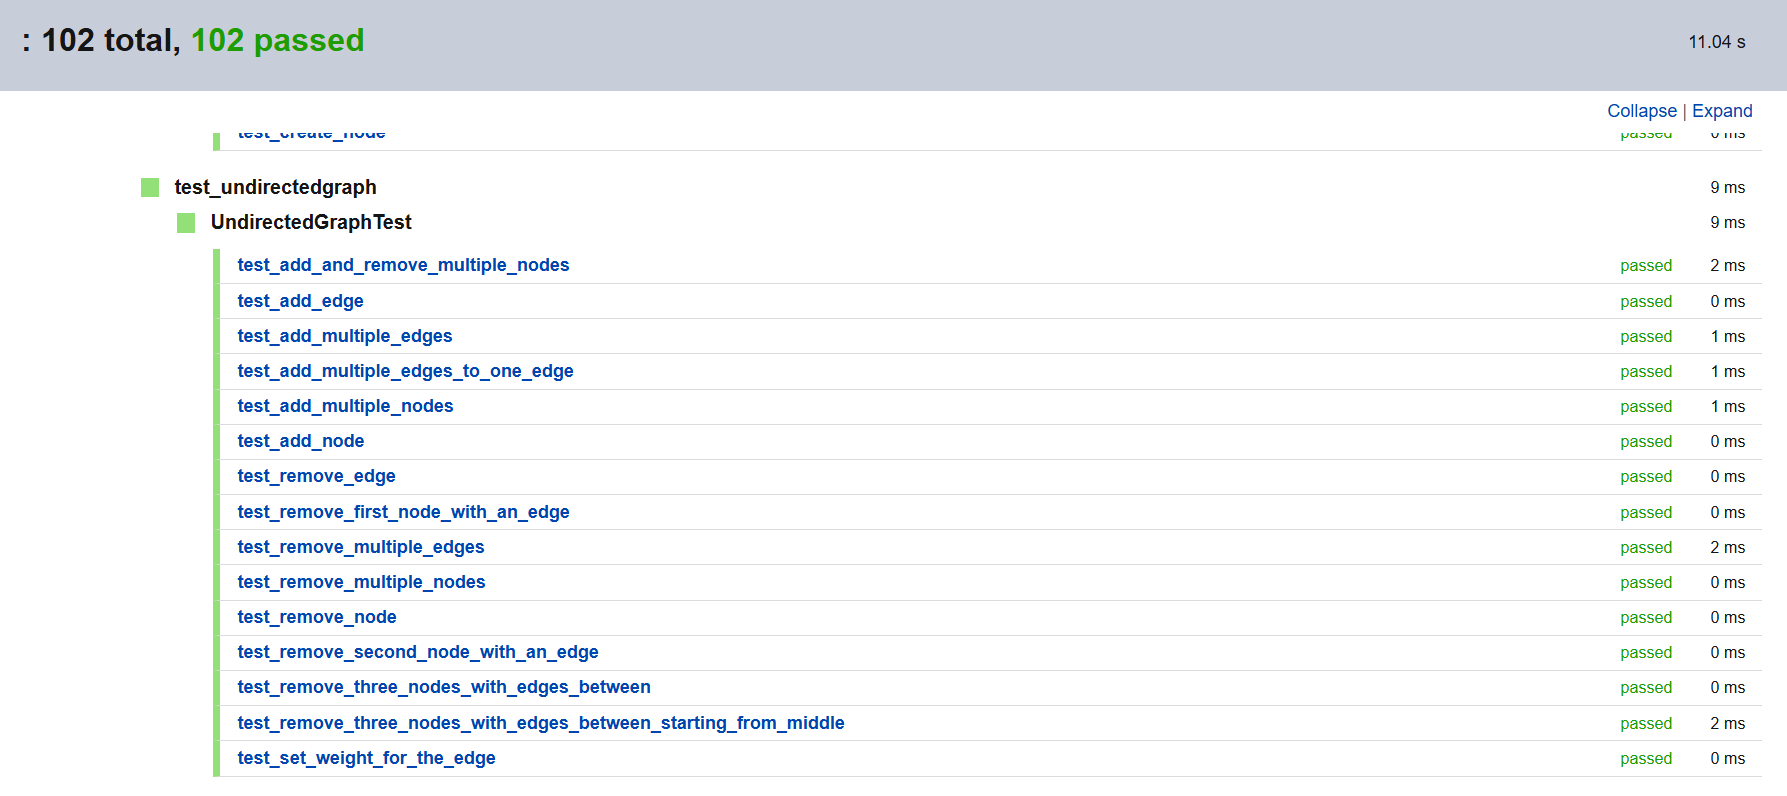
\includegraphics[width=\textwidth]{images/tests_pass.png}
	\caption{Unit tests passing}
\end{figure}

\begin{figure}[H]
	\centering
	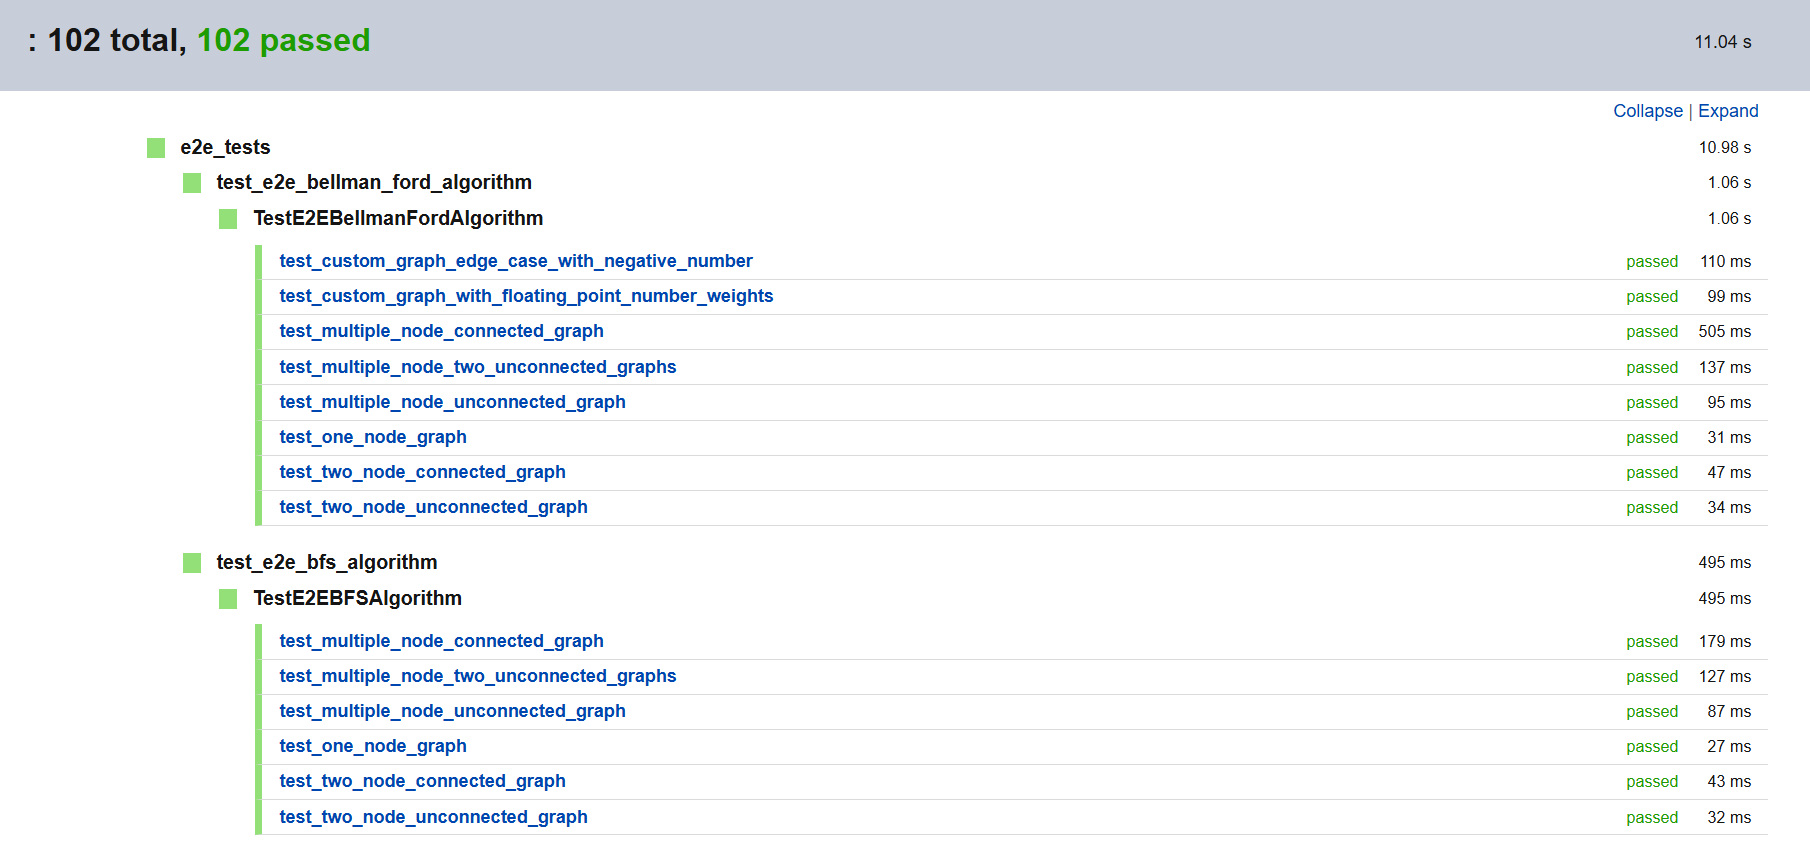
\includegraphics[width=\textwidth]{images/e2e_tests_pass.png}
	\caption{E2E tests passing}
\end{figure}